\chapter{Tesseroides de densidad variable}
\label{cha:tesseroids-variable-density}

Este capítulo es una traducción al Español del artículo titulado
\emph{Gravitational field calculation in spherical coordinates using variable
densities in depth} escrito por Santiago R. Soler, Agustina Pesce, Mario E.
Gimenez y Leonardo Uieda, y publicado en \emph{Geophysical Journal
International} en Junio de 2019 \citep{soler2019}.
Una preimpresión del artículo se encuentra disponible bajo licencia Creative
Commons Atribución 4.0 Internacional en
\href{https://eartharxiv.org/}{EarthArXiv} (doi:
\href{https://doi.org/10.31223/osf.io/3548g}{10.31223/osf.io/3548g}).

\section{Resumen}

Presentamos una nueva metodología para calcular los campos gravitatorios
generados por tesseroides (prismas esféricos) cuya densidad varía en
profundidad según una función continua arbitraria.
Esta metodología aproxima los campos gravitatorios mediante una \ac{GLQ} junto
con la aplicación de dos algoritmos de discretización que controlan
automáticamente la precisión de la aproximación dividiendo adaptativamente el
tesseroide original en otros más pequeños.
El primero es un algoritmo preexistente de discretización adaptativa
bidimensional que reduce el error debido a la distancia entre el tesseroide
y el punto de cómputo.
El segundo es un nuevo algoritmo de discretización basado en la densidad que
reduce los errores debido a la variación de la densidad con la profundidad.
La cantidad de subdivisiones que realiza cada algoritmo es indirectamente
controlada por dos parámetros: el \emph{ratio distancia-tamaño} y el
\emph{ratio delta}.
Hemos obtenido soluciones analíticas de los campos gravitatorios generados por
un cascarón esférico con densidades variables a lo largo de la dirección radial
y los hemos comparado con los resultados del modelo numérico para densidades
lineales, exponenciales y sinusoidales.
Las densidades oscilantes fueron utilizadas con la única intención de someter
al algoritmo a sus límites y no para emular un escenario real.
Estas comparaciones nos han permitido obtener valores óptimos para los ratio
distancia-tamaño y delta que garantizan una precisión de 0.1\% en relación con
las soluciones analíticas.
Los valores óptimos del ratio distancia-tamaño para el potencial gravitatorio
y su gradiente son 1 y 2.5, respectivamente.
La discretización basada en la densidad no produce subdivisiones en el caso de
densidad lineal, pero un ratio delta de 0.1 es necesario para densidades
exponenciales y para la mayoría de las sinusoidales.
Estos valores pueden ser extrapolados para cubrir los usos más comunes, los
cuales son siempre más sencillos que perfiles de densidad que oscilan.
Sin embargo, los ratios densidad-tamaño y delta pueden ser configurados por el
usuario para aumentar la precisión de los resultados a expensas de un aumento
en el tiempo de cómputo.
Por último, hemos aplicado esta nueva metodología para modelar la Cuenca
Neuquina, una cuenca de antepaís en Argentina, con una profundidad máxima de
5000~m y utilizando una densidad exponencial.


\section{Introducción}

La variación de la densidad de la litósfera con la profundidad ha sido
estudiada por casi un siglo.
A lo largo de este tiempo, varias relaciones entre la densidad y la profundidad
han sido propuestas para diferentes tipos de rocas
\citep[por ejemplo~][]{maxant1980, rao1986, rao1993, rao1994}.
Además, densidades que varían con la profundidad han sido utilizadas en el
modelado directo e inverso de datos gravitatorios, principalmente aplicados
a cuencas sedimentarias
\citep{cordell1973, rao1986, cowie1990, rao1993, rao1994, zhang2001,
welford2010}.
Estos modelos directos han sido desarrollados para cuerpos bidimensionales
o tridimensionales en coordenadas Cartesianas, lo que limita su aplicación
a escalas locales.
La llegada de la gravimetría satelital ha proveído mediciones del campo
gravitatorio terrestre con cobertura global, permitiendo el modelado
e interpretación en escalas regionales o globales.
Por esta razón, diseñar métodos de modelado directo que reproducen las
anomalías de gravedad para esas escalas resulta muy importante.

Con el objetivo de tomar en consideración la curvatura de la Tierra, muchos
modelos directos globales se definen en coordenadas esféricas geocéntricas
(ver Capítulo~\ref{cha:fundamentos}).
Un abordaje común es discretizar la Tierra en tesseroides \citep{anderson1976},
es decir prismas esféricos, los cuales son definidos por el volumen que
delimitan pares de latitud, longitud y radios (Fig.~\ref{fig:tesseroid}).
Los campos gravitatorios generado por un tesseroide en cualquier punto exterior
vienen dados por integrales de volumen que deben ser aproximadas numéricamente.
La literatura ofrece dos abordajes principales: uno involucra expansiones en
series de Taylor \citep{heck2006, grombein2013}, mientras que la otra hace uso
de la \ac{GLQ}
La expansión en series de Taylor no resulta adecuada para desarrollar un
algoritmo para densidades variables según funciones arbitrarias.
Los diferentes términos de las series deberían obtenerse para cada una de las
posibles funciones de densidad.
Por el contrario, una función de densidad arbitraria puede incluirse dentro de
la \ac{GLQ} sin necesidad de modificar el método de integración.
Es por esta razón que haremos foco en los métodos basados en la \ac{GLQ} de
aquí en adelante.

El principal desafío de la integración por \ac{GLQ} es la pérdida de precisión
que ocurre cuando el punto de cómputo se acerca al tesseroide \citep{ku1977}.
\citet{uieda2016} desarrollaron un método a partir del algoritmo de
discretización adaptativa tridimensional de \citet{li2011} para obtener de
manera automática campos gravitatorios de tesseroides con densidad uniforme con
0.1\% de precisión.
El algoritmo divide recursivamente un tesseroide en otros más pequeños cuando
un determinado umbral es excedido, esto es cuando la distancia normalizada
entre el punto de cómputo es mayor que un parámetro denominado \emph{ratio
distancia-tamaño} ($D$).
\citet{uieda2016} obtuvieron además valores estándar de $D$ para el cómputo del
potencial gravitatorio, las componentes de su gradiente y del tensor de Marussi
comparando los resultados de la integración numérica con los campos generados
por un cascarón esférico.

Dos publicaciones recientes presentan abordajes alternativos para calcular los
campos gravitatorios de tesseroides homogéneos e incorporan metodologías para
el caso de tesseroides con densidades variables en profundidad.
\citet{fukushima2018} ha resuelto analíticamente la integral correspondiente al
potencial gravitatorio en la dirección radial, obteniendo una integral de
superficie, la cual es posteriormente resuelta dividiendo condicionalmente el
tesseroide y aplicando la cuadratura exponencial doble.
El gradiente del potencial y las componentes del tensor de Marussi son
calculadas posteriormente por diferencias finitas.
\citet{fukushima2018} además generaliza el método para tesseroides con una
densidad que varía con el radio según una función polinomial de grado
arbitrario.
\citet{lin2019} han comparado las diferentes metodologías de integración
y discretización para tesseroides homogéneos.
A partir de este análisis han desarrollado un método combinado:
Para puntos de cómputo cercanos al tesseroide, utilizan una integración
\ac{GLQ} junto con una discretización adaptativa basada en \citet{uieda2016}
pero solo aplicada a las dimensiones horizontales.
Si el punto de cómputo se encuentra más allá de una cierta distancia de
truncamiento, aplican una aproximación en serie de Taylor de segundo orden,
junto con la subdivisión desarrollada por \citet{grombein2013}.
\citet{lin2019} además introducen una variación de su método combinado para
calcular los campos gravitatorios generados por tesseroides con densidades
lineales en la dirección radial.

Los desarrollos de \citet{lin2019} y \citet{fukushima2018} se limitan
a funciones de densidad polinomiales.
Si bien la mayoría de las funciones suaves pueden aproximarse por funciones
lineales de a pasos, la elección del intervalo de discretización no es ni
directa ni automática para el caso general.
Aunque existen muchos algoritmos de aproximación lineales de a pasos
automatizan este proceso \citep{ketkov1969, vandewalle1975, imamoto2008,
ahmadi2013}, requieren un número fijo de intervalos de discretización o están
diseñados para ser utilizados solo en funciones convexas.
El uso de estos algoritmos limitaría el dominio de funciones de densidades que
pueden ser asignadas a tesseroides y no garantizarían un proceso completamente
automático.
Además, es bien conocido que el uso de polinomios de alto grado para aproximar
una función altamente variable produce resultados inestables cuando se
extrapola más allá del dominio de datos.
Estos obstáculos podrían hacer que aproximar densidades mediante aproximaciones
lineales de a pasos o por polinomios de alto grado no resulte adecuado para
inversiones de gravedad no lineales \citep[e.g.][]{uieda2017} si la función
densidad es altamente variable en profundidad.

Presentamos un nuevo algoritmo para el cálculo del potencial gravitatorio y su
gradiente generado por un tesseroide con una función continua de densidad sobre
cualquier punto de cómputo externo.
Esta metodología está basada en una integración \ac{GQL} tridimensional, una
versión bidimensional del algoritmo de discretización adaptativa de
\citet{uiedauieda2016} (de acuerdo con \citet{lin2019}), y un nuevo algoritmo
de discretización basado en la densidad.
Para garantizar la precisión de la aproximación numérica, hemos determinado
empiricamente valores óptimos para los parámetros que controlan las
discretizaciones, comparando los resultados numéricos con las soluciones
analíticas de cascarones esféricos.
Finalmente, hemos aplicado la nueva metodología para modelar la Cuenca
Neuquina, Argentina, utilizando tesseroides con densidades lineales
y exponenciales en profundidad.

%%%%%%%%%%%%%%%%%%%%%%%%%%%%%%%%%%%%%%%%%%%%%%%%%%%%%%%%%%%%%%%%%%%%%%%%%%%%%%

\section{Methodology}

Consider a tesseroid in a geocentric spherical coordinate system defined by
pairs of geocentric latitudinal ($\phi_1$, $\phi_2$), longitudinal ($\lambda_1$,
$\lambda_2$), and radial ($r_1$, $r_2$) boundaries.
We define an external computation point $P(r, \phi, \lambda)$ located at radius $r$,
geocentric latitude $\phi$, and longitude $\lambda$.
\citet{grombein2013} provide efficient formulations for the volume integrals of the
gravitational potential and its first- and second-order derivatives of a tesseroid with
homogeneous density.
The derivatives of the gravitational potential are taken with
respect to the local north-oriented Cartesian coordinate system with origin at $P$
(Fig.~\ref{fig:tesseroid}).
Here, we will assume that the tesseroid has a density varying with $r$ according to an
arbitrary continuous function $\rho(r)$.
Thus, the integrals for the gravitational potential and its first-order derivatives are
slightly modified to

\begin{equation}
    V(r,\phi,\lambda) = G
    \int\limits_{\lambda_1}^{\lambda_2}
    \int\limits_{\phi_1}^{\phi_2}
    \int\limits_{r_1}^{r_2}
    \frac{\rho(r')}{\ell} \kappa \,  dr' d\phi' d\lambda',
\label{eq:tesseroid-pot}
\end{equation}

\noindent and

\begin{equation}
    g_{\alpha}(r,\phi,\lambda) = G
    \int\limits_{\lambda_1}^{\lambda_2}
    \int\limits_{\phi_1}^{\phi_2}
    \int\limits_{r_1}^{r_2}
    \rho(r') \frac{\Delta_\alpha}{\ell^3}
    \kappa \, dr' d\phi' d\lambda',
\label{eq:tesseroid-grav}
\end{equation}

\noindent in which $\alpha \in \{x, y, z\}$,
$G = 6.674\times10^{-11}\, \text{m$^3$kg$^{-1}$s$^{-1}$}$ is the gravitational constant
and

\begin{equation}
    \Delta_x = r'[\cos\phi\sin\phi' - \sin\phi\cos\phi'
               \cos(\lambda' - \lambda)],
\end{equation}
\begin{equation}
    \Delta_y = r' \cos \phi' \sin(\lambda' - \lambda),
\end{equation}
\begin{equation}
    \Delta_z = r' \cos \psi - r,
\end{equation}
\begin{equation}
    \kappa = {r'}^2 \cos \phi',
\end{equation}
\begin{equation}
    \ell = \sqrt{{r'}^2 + r^2 - 2 r r' \cos \psi},
\label{eq:ell}
\end{equation}
\begin{equation}
    \cos\psi = \sin\phi\sin\phi' + \cos\phi\cos\phi'
                 \cos(\lambda' - \lambda).
\label{eq:cospsi}
\end{equation}


\subsection{Gauss-Legendre Quadrature integration}

Applying a $N$th order GLQ, we can approximate each integral in
equations~\ref{eq:tesseroid-pot} and~\ref{eq:tesseroid-grav} by a weighted sum of the
integration kernel evaluated on the roots of an $N$th order Legendre polynomial
\citep[p.~390]{hildebrand1987}.
Unlike the homogeneous density case, the radial density function $\rho(r)$ must also be
included in the integration and evaluated on the Legendre polynomial roots
(i.e.~quadrature nodes).

%\iftwocol{
\begin{equation}
    \begin{split}
        \int\limits_{\lambda_1}^{\lambda_2}
        \int\limits_{\phi_1}^{\phi_2}
        \int\limits_{r_1}^{r_2}
        \rho(r') f(r', \phi', \lambda')
        dr' d\phi' d\lambda' \approx& \\
        A
        \sum\limits_{i=1}^{N^r}
        \sum\limits_{j=1}^{N^\phi}
        \sum\limits_{k=1}^{N^\lambda}
        W_i^r W_j^\phi W_k^\lambda
        &\rho(r_i) f(r_i, \phi_j, \lambda_k),
    \end{split}
\label{eq:glq-var-dens}
\end{equation}
%}{
%\begin{equation}
    %\int\limits_{\lambda_1}^{\lambda_2}
    %\int\limits_{\phi_1}^{\phi_2}
    %\int\limits_{r_1}^{r_2}
    %\rho(r') f(r', \phi', \lambda')
    %dr' d\phi' d\lambda' \approx
    %A
    %\sum\limits_{i=1}^{N^r}
    %\sum\limits_{j=1}^{N^\phi}
    %\sum\limits_{k=1}^{N^\lambda}
    %W_i^r W_j^\phi W_k^\lambda \rho(r_i) f(r_i, \phi_j, \lambda_k),
%\label{eq:glq-var-dens}
%\end{equation}
%}

\noindent where

\begin{equation}
    A = \frac{(\lambda_2 - \lambda_1)(\phi_2 - \phi_1)(r_2 - r_1)}{8},
\end{equation}

\noindent $f(r', \phi', \lambda')$ is an integral kernel for a homogeneous tesseroid
\citep{grombein2013},
$(r_i, \phi_j, \lambda_k)$ are the coordinates of the quadrature nodes,
$N^r$, $N^\phi$, $M^\lambda$ are the quadrature orders and $W_i^r$, $W_j^\phi$,
$W_k^\lambda$ are the quadrature weights in the radial, latitudinal, and longitudinal
directions, respectively.
\citet[p.~391]{hildebrand1987} provides the formulas for calculating the GLQ weights and
pre-computed values of the Legendre polynomial roots for low orders.
See \citet{uieda2016} for a more detailed description using a similar notation to the
one used here.
It is worth noting that a GLQ is equivalent to approximating the tesseroid by $N^r
\times N^\phi \times N^\lambda$ point masses located on the quadrature nodes
\citep{ku1977, asgharzadeh2007}.


\subsection{Two Dimensional Adaptive Discretization}

\citet{ku1977} noticed that the GLQ integration
becomes less accurate when the computation point is closer to the
mass element.
One way to prevent this from happening would be to increase the GLQ order.
Doing so would uniformly increase the number of point masses inside the
tesseroid volume.
However, an increase in the point mass concentration is only required close to the
computation point \citep{uieda2016}.
Alternatively, \citet{li2011} proposed an adaptive
discretization algorithm which keeps the GLQ order fixed and divides the
tesseroid based on a ratio between the distance to the computation
point and its dimensions.
This algorithm produces a more efficient computation because an increased concentration
of point masses is produced where it is needed more.
\citet{uieda2016} developed a modified version of this algorithm along with an efficient
computational implementation.
Both algorithms perform tesseroid subdivisions in the latitudinal,
longitudinal and radial directions, thus we can define them as three-dimensional
adaptive discretization algorithms.
On the other hand, \citet{lin2019} proposed a two dimensional discretization algorithm
that subdivides the tesseroid only on the latitudinal and longitudinal directions.
Removing a dimension from the discretization makes the computation more efficient by
reducing the number of tesseroids in the model, while
retaining an acceptable accuracy \citep{lin2019}.

Here we will follow \citet{lin2019} and use a two dimensional version of the adaptive
discretization of \citet{uieda2016}.
What follows is a summary of the algorithm and the reader is referred to
\citet{uieda2016} for a detailed description.

\textit{Step 1}: Check that the tesseroid satisfies the following inequality for its
latitudinal and longitudinal dimensions $L_i\ (i \in \{\lambda, \phi\})$:

\begin{equation}
    \frac{d}{L_i} \geq D,
    \label{eq:condition}
\end{equation}

\noindent
in which $D$ is a positive scalar called the distance-size ratio, $d$ is the distance
between the computation point and the geometric centre of the tesseroid

\begin{equation}
    d = \left[
        r^2 + r_t^2 - 2 r r_t \cos\psi_t
        \right]^{\frac{1}{2}} ,
    \label{eq:distance}
\end{equation}

\begin{equation}
    \cos\psi_t =
        \sin\phi\sin\phi_t + \cos\phi\cos\phi_t\cos(\lambda - \lambda_t),
\end{equation}

\begin{equation}
    r_t = \frac{r_2 + r_1}{2}, \quad
    \phi_t = \frac{\phi_2 + \phi_1}{2}, \quad
    \lambda_t = \frac{\lambda_2 + \lambda_1}{2},
\end{equation}

\noindent
and the dimensions of the tesseroid are defined as

\begin{equation}
    L_\lambda = r_2 \arccos(\sin^2\phi_t +
        \cos^2\phi_t\cos(\lambda_2 - \lambda_1)),
    \label{eq:sizelon}
\end{equation}

\noindent and

\begin{equation}
    L_\phi = r_2 \arccos(\sin\phi_2\sin\phi_1 + \cos\phi_2\cos\phi_1).
\end{equation}

\textit{Step 2}:
If none of the dimensions of the tesseroid fail inequality~\ref{eq:condition}, then
compute the gravitational effect of the tesseroid using a second-order GLQ
(Eq.~\ref{eq:glq-var-dens}).
Add the computed effect to a running total.

\textit{Step 3}:
If inequality~\ref{eq:condition} does not hold for one of the dimensions
(longitudinal or latitudinal), split the tesseroid in half along that dimension.
Repeat steps 1-3 for all smaller tesseroids until none are left that violate
inequality~\ref{eq:condition}.

\textit{Final step}:
By the end of the algorithm, a second-order GLQ will have been applied to each smaller
tesseroid and the running total gathered in step 2 will be the gravitational effect of
the original tesseroid.

The distance-size ratio $D$ determines how many times the tesseroids will be divided.
Therefore, it effectively regulates both the accuracy of the algorithm and its
computation time.
An optimal value for $D$ cannot be directly calculated from the desired accuracy level.
Instead, it is empirically determined by comparing the numerical results with the
analytical solution for a spherical shell.
\citet{uieda2016} used a shell with homogeneous density to determine optimal values of
$D$.
Here, we will repeat the numerical experiment using analytical expressions for shells
with density varying according to functions of $r$.
This experiment will also test whether the same values of $D$ determined by
\citet{uieda2016} can be used for the two dimensional adaptive discretization.


\subsection{Density-based Discretization Algorithm}

\begin{figure*}
\centering
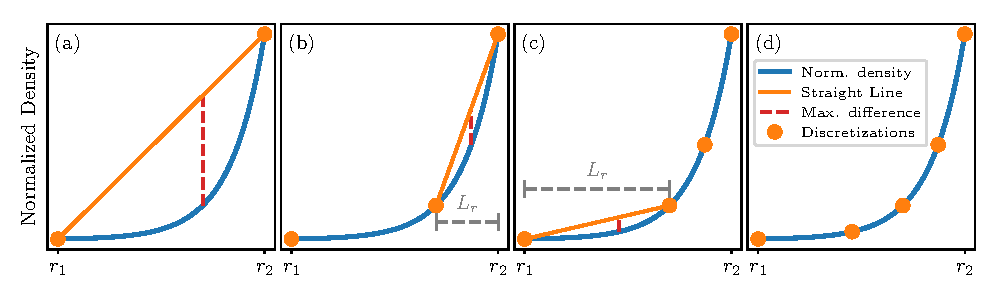
\includegraphics[width=\linewidth]
    {figs/tesseroids-variable-density/density-based-discretization-algorithm.pdf}
\caption{
    Example application of the density-based discretization algorithm to a non-linear
    density function.
    (a)~The normalised density function $\rho_n(r')$ (blue), current boundaries of the
    tesseroid (orange dots), and the straight line $\rho_l(r')$ (orange line).
    The dashed red line represents the maximum density difference $\Delta \rho (r')$ at
    which the tesseroid would be divided (assuming that the
    inequality~\ref{eq:delta-density} is not satisfied).
    (b)~Second iteration of the algorithm with a new straight line and maximum
    density difference. The tesseroid would be divided at the depth indicated by the
    dashed red line.
    (c)~Third iteration of the algorithm.
    (d)~Final output of the density-based discretization, assuming that all four new
    tesseroids satisfy inequality~\ref{eq:delta-density}.
}
\label{fig:density-discretization-algorithm}
\end{figure*}

The numerical integration of an arbitrary continuous density function introduces a new
type of problem: the integration error from using only a few quadrature nodes to account
for the variation of the density function.
The three dimensional adaptive discretization may help to reduce this kind of error by
adding more point masses in the radial direction.
However, it does not take into account the density function itself when dividing the
tesseroid and hence it is not well suited to fully perform this task.

We have developed a complementary discretization algorithm in the radial direction that
takes into account the variations of the density function.
This density-based discretization is applied prior to the two dimensional adaptive
discretization described in the previous section.
In short, the algorithm divides the tesseroid along the radial dimension at the
depths at which the \emph{maximum density variations} take place.

Consider an \emph{original} tesseroid with a density given by the continuous function
$\rho(r')$.
Before the density-based discretization starts,
we normalise the density function to the range $[0, 1]$ as follows

\begin{equation}
    \rho_n(r') =
    \frac{\rho(r') - \rho_\text{min}}{\rho_\text{max} - \rho_\text{min}},
\end{equation}

\noindent in which $\rho_\text{min}$ and $\rho_\text{max}$ are the minimum and maximum
density values inside the tesseroid boundaries.
We emphasize that this normalised density function will not be modified throughout the
algorithm.
In case the density function is constant, both maximum and minimum densities will be
equal and the density-based discretization algorithm will not be applied.

The algorithm is comprised of the following steps
(Fig.~\ref{fig:density-discretization-algorithm}):

\textit{Step 1}:
Define a straight line $\rho_l(r')$ that assumes the same values as the normalised
density function $\rho_n(r')$ at the boundaries of the tesseroid ($r_1$ and $r_2$):

\begin{equation}
    \rho_l(r') =
    \frac{ \rho_n(r_2) - \rho_n(r_1) }{ r_2 - r_1 } (r' - r_1) + \rho_n(r_1).
    \label{eq:density-reference-line}
\end{equation}

\textit{Step 2}:
Evaluate the normalised density function and the straight line on a range of $N$ radii
between $r_1$ and $r_2$.
We have opted for $N = 101$ but the specific value of $N$ is not critical to the
algorithm.

\textit{Step 3}:
Compute the absolute difference between the values of the straight line and the
normalised density function:

\begin{equation}
    \Delta \rho (r') = | \rho_n(r') - \rho_l(r') |.
    \label{eq:density-abs-diff}
\end{equation}

\textit{Step 4}:
If the following inequality holds, the tesseroid will not be divided:

\begin{equation}
    \text{max}\{ \Delta \rho(r') \} \frac{L_r}{L_r^\text{orig}} \le \delta,
    \label{eq:delta-density}
\end{equation}

\noindent
in which $L_r$ is the radial dimension of the tesseroid being considered for division,

\begin{equation}
    L_r = r_2 - r_1,
\end{equation}

\noindent $L_r^\text{orig}$ is the radial dimension of the original tesseroid, and
$\delta$ is a positive constant henceforth called the \textit{delta ratio}.

\textit{Step 5}:
If inequality~\ref{eq:delta-density} is not satisfied, then the tesseroid is split in
two parts at the radius $r_\text{max}$ at which the maximum absolute difference
(Eq.~\ref{eq:density-abs-diff}) takes place.
Repeat steps 1-5 for each smaller tesseroid produced in this step.

\textit{Final step}:
Once all smaller tesseroids satisfy inequality.~\ref{eq:delta-density}, each one is
subjected to the two dimensional adaptive discretization algorithm described earlier to
calculate their gravitational effects.

On the first iteration, the ratio $L_r/L_r^\text{orig}$ equals one because the tesseroid
being divided is the original one.
For further iterations, the ratio will be progressively smaller than one as the
tesseroids get smaller.
This is intended to limit the number of divisions to the ones that will
significantly reduce the numerical error:
dividing a large tesseroid with a small $\text{max}\{ \Delta \rho(r') \}$ would
improve the integration accuracy more than dividing a small tesseroid with a
higher $\text{max}\{ \Delta \rho(r') \}$.

The higher $\delta$ is, the fewer divisions will be made, and vice-versa.
Thus, it controls how many times the tesseroids will be divided based on the density
function and, indirectly, determines the accuracy and computation time of
numerical integration.
This raises the need to determine a maximum value of $\delta$ that
ensures an acceptable accuracy while minimising the computation time.


\subsection{Algorithm summary}

In summary, given a tesseroid with density varying in depth according to an arbitrary
continuous function, we propose the following steps to numerically compute its
gravitational fields on an external point:

\textit{Step 1:}
Apply the density-based discretization algorithm to discretize the tesseroid in the
radial dimension, producing a set of tesseroids with the same longitudinal and
latitudinal dimensions as the original one but with different radial boundaries.

\textit{Step 2:}
Apply the two dimensional adaptive discretization algorithm for each tesseroid obtained
in the previous step.
If needed, the algorithm will divide each tesseroid in the latitudinal and longitudinal
direction, generating a set of smaller tesseroids.

\textit{Step 3:}
Apply a second-order GLQ to numerically compute the gravitational fields
(Eq.~\ref{eq:glq-var-dens}) generated by each tesseroid obtained in the
previous step.
The numerical integration includes the density function and can be applied
without modification to any continuous function.
The sum of these results is the gravitational field of the original tesseroid.


\subsection{Software implementation}

We have implemented the algorithms described in the previous sections in the Python
programming language.
The software is based on the Python implementation of \citet{uieda2016} that is included
in the Fatiando a Terra library v0.5 \citep{uieda2013}.
The more time consuming parts of the algorithm are written in the Cython language to
achieve higher performance.
We leverage the dynamic nature of the Python language to allow user-defined radial
density functions as inputs to the software.
Thus, our code can evaluate linear, exponential, polynomial, sinusoidal, cubic splines,
or any other continuous density function without modification.
This new code is freely available under the BSD 3-clause open-source license.
All source code, Python scripts, data, and model results are made available through
an online repository
\href{https://doi.org/10.6084/m9.figshare.8239622}{doi.org/10.6084/m9.figshare.8239622}
\citep{soler2019b} or
\href{https://github.com/pinga-lab/tesseroid-variable-density}{github.com/pinga-lab/tesseroid-variable-density}.
The repository also contains instructions for replicating all results
presented here.



%%%%%%%%%%%%%%%%%%%%%%%%%%%%%%%%%%%%%%%%%%%%%%%%%%%%%%%%%%%%%%%%%%%%%%%%%%%%%

\section{Determination of the distance-size and delta ratios}

The distance-size ratio $D$ of the adaptive discretization and the delta ratio $\delta$
of the density-based discretization determine how many times each tesseroid will be
divided and thus indirectly control the numerical error of the integration.
Optimal values for $D$ and $\delta$ must be determined in order to ensure both
acceptable numerical accuracy and computation efficiency for the algorithm.

\citet{uieda2016} compared the numerical integration of homogeneous density tesseroids
with the analytical solution of a spherical shell \citep{mikuska2006, grombein2013} in
order to obtain default values for the distance-size ratio $D$.
We will follow this idea but for our needs the spherical shell must
have the same density function of radius as our tesseroid model.
\citet{lin2019} show the analytical solution of the gravitational potential generated by
a spherical shell with linear density in the radial coordinate.
Applying the Newton's Shell Theorem \citep{chandrasekhar1995, binney2008},
we derive expressions for the gravitational potential of a spherical shell with
linear, exponential, and sinusoidal density functions
(see Appendix~\ref{cha:shell}).

In order to compare the numerical results with the analytical solution we must build
spherical shell models out of tesseroids.
We divide the spherical shell along the latitudinal and longitudinal directions to
obtain a shell model made out of $6 \times 12 = 72$ tesseroids of size
$30^\circ \times 30^\circ$.
In order to asses the density-based discretization in the radial dimension,
we use spherical shell models with different thicknesses (Table~\ref{tab:shell-models}).
The thickness values were chosen to represent a range of applications, from topographic
to lithospheric scale models.
Because the amount of tesseroid divisions in the adaptive discretization will be
proportional to the tesseroid size (Eq.~\ref{eq:condition}),
some of these configurations represent worse-case scenarios.
Most practical applications will use tesseroids smaller than
$30^\circ \times 30^\circ \times 1000\ \text{km}$.

The differences between the analytical and numerical solutions could be calculated on a
single computation point due to the rotational symmetry of the spherical shell.
However, the numerical results depend on the relative location between the computation
point and the tesseroid \citep{ku1977, asgharzadeh2007, uieda2016}.
We account for this effect by calculating the differences on regular grids and keeping
only the maximum absolute difference.
All calculations are repeated for four different computation grids
(Table~\ref{tab:grids}):
a local grid at the pole, a local grid at the equator, a global grid at zero height
above the shell, and a global grid at a height of 260 km (representing the nominal
height of the GOCE satellite).
These grids span a broad scenario of use cases and ensure an acceptable accuracy on each
one of them.

We perform comparisons between the analytical solutions for the spherical shell and the
numerical integration results for linear, exponential, and sinusoidal density
functions.
The sinusoidal density case is included in order to test the numerical approximation to
its limits.
The comparisons are repeated for all combinations of tesseroid models in
Table~\ref{tab:shell-models} and computation grids in Table~\ref{tab:grids}.
From these results, we generalize optimal values for $D$ and $\delta$ that ensure a
numerical error lower than 0.1\% of the spherical shell values for most use cases.

\begin{table}
\caption{
    Description of the tesseroid models used to build spherical shells and characterize
    the accuracy of the numerical integration.
    The outer radius ($R_2$) of every shell model is equal to the mean Earth radius
    (6378.137 km), while the inner radius ($R_1$) is determined by its thickness.
    The horizontal dimensions of the tesseroids and the total number of
    tesseroids in the shell model are given in the latitudinal and longitudinal
    dimensions, respectively.
    \newline
}
\label{tab:shell-models}
\centering
\begin{tabular}{rccccc}
    Thickness & Tesseroid size & Number of tesseroids \\ \hline
    0.1 km  & $30^\circ \times 30^\circ$ & $6 \times 12 = 72$ \\
    1 km    & $30^\circ \times 30^\circ$ & $6 \times 12 = 72$ \\
    10 km   & $30^\circ \times 30^\circ$ & $6 \times 12 = 72$ \\
    100 km  & $30^\circ \times 30^\circ$ & $6 \times 12 = 72$ \\
    1000 km & $30^\circ \times 30^\circ$ & $6 \times 12 = 72$ \\
\end{tabular}
\end{table}

\begin{table*}
\caption{
    Description of the computation grids used to characterize the accuracy of the
    numerical integration.
    Grid height is defined above the mean Earth radius.
    \newline
}
\label{tab:grids}
\centering
\begin{tabular}{lccc}
    Name & Grid spacing & Grid region (degrees) & Grid height (km)
    \\ \hline
    Pole      & $0.1^\circ$ &   0E /   1E / 89N / 90N & 0   \\
    Equator   & $0.1^\circ$ &   0E /   1E /  0N / 1N  & 0   \\
    Global    & $ 10^\circ$ & 180W / 180E / 90S / 90N & 0   \\
    Satellite & $ 10^\circ$ & 180W / 180E / 90S / 90N & 260 \\
\end{tabular}
\end{table*}


\subsection{Linear Density}

A spherical shell with a linear density function given by

\begin{equation}
    \rho(r') = ar' + b,
    \label{eq:density-linear}
\end{equation}

\noindent
has an analytical solutions for the gravitational potential and its vertical derivative
given by Eqs.~\ref{eq:shell-pot-linear} and~\ref{eq:shell-gz}.
The values of the angular and linear coefficients ($a$ and $b$)
can be chosen so that the density assumes the values of $\rho_\text{in} = 3300$~kg/m$^3$
and $\rho_\text{out} = 2670$~kg/m$^3$ on the inner ($R_\text{in}$) and outer
($R_\text{out}$) radii of the shell, respectively,

\begin{equation}
    a = \frac{\rho_\text{out} - \rho_\text{in}}{R_\text{out} - R_\text{in}},
\end{equation}

\begin{equation}
    b = \rho_\text{out} -
    \frac{\rho_\text{out} - \rho_\text{in}}{R_\text{out} - R_\text{in}} R_\text{out}.
\end{equation}


\begin{figure*}
\centering
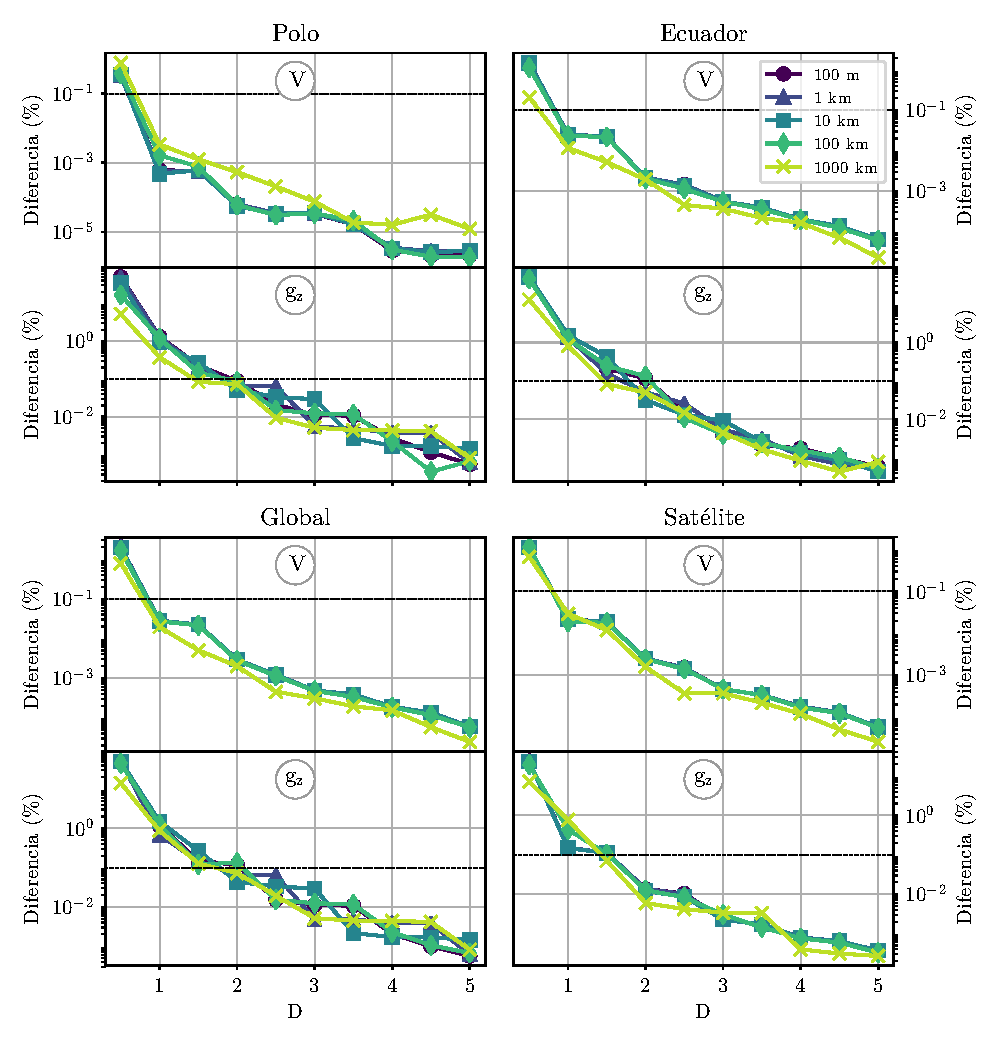
\includegraphics[width=\linewidth]{figs/tesseroids-variable-density/linear-density-diffs.pdf}
\caption{
    Differences between the gravitational fields generated by each tesseroid shell model
    and the analytical solution as a function of the distance-size ratio $D$.
    Each model has a linear density function (Eq.~\ref{eq:density-linear}).
    The computations were performed on the four grids described in Table~\ref{tab:grids}
    and using the shell models detailed in Table~\ref{tab:shell-models}.
    Each line represents the maximum absolute difference between the numerical results
    and the analytical solution for a given shell model.
    Due to the linearity of the density function, the density-based discretization
    algorithm is not applied.
    Differences are reported as a percentage of the analytical solutions.
    The horizontal dashed black line represents a target difference of 0.1\%.
}
\label{fig:D-linear}
\end{figure*}

The absolute density difference defined on equation~\ref{eq:density-abs-diff} will
always be zero for the linear density case.
As a result, the inequality~\ref{eq:delta-density} will always be satisfied and no
divisions will ever be performed during the density-based discretization.
Therefore, the two dimensional adaptive discretization algorithm is the
only mechanism that controls the accuracy of the numerical integration for the linear
density case.
For this reason, we will ignore the values of $\delta$ and only determine the minimum
value of $D$ needed in order to guarantee an acceptable accuracy.

We compute the gravitational potential ($V$) and its vertical derivative ($g_z$) for
each shell model in Table~\ref{tab:shell-models} on each computation grid in
Table~\ref{tab:grids}.
The horizontal derivatives of the potential are equal to zero outside of the shell due
to the rotational symmetry and are thus omitted from the analysis.
The computations are repeated for values of the distance-size ratio $D$ ranging from 0.5
to 5 in increments of 0.5.
We then calculate the absolute difference between the numerical results and the
analytical solution for the shell.
Fig.~\ref{fig:D-linear} shows the maximum absolute difference for each shell model and
computation grid as a function of $D$.
The differences are relative to the shell value.
Finally, we set the optimal value of $D$ as the smallest value for which the difference
is below 0.1\%.

We observe from Fig.~\ref{fig:D-linear} that the relative errors for the potential and
$g_z$ fall below the 0.1\% threshold at $D=1$ and $D=2.5$, respectively.
Notably, a value of $D=2$ would suffice for $g_z$ in the case of the satellite height
grid.
For all other configurations, these values are consistent and independent of the shell
model thickness or geographic location.


\subsection{Exponential Density}

For an exponential density function, the density-based discretization will be applied
before the adaptive discretization algorithm.
This means that optimal values for both the distance-size ratio $D$ and the delta ratio
$\delta$ (Eq.~\ref{eq:delta-density}) must be determined.
We perform an error analysis similar to what was done for the linear density case.
Now the spherical shell will have an exponential density function that assumes the
values of $\rho_\text{out} = 2670$~kg/m$^3$ and $\rho_\text{in} = 3300$~kg/m$^3$ on the
outer and inner surfaces, respectively, defined as follows:

\begin{equation}
    \rho(r') = A e^{- b \frac{r' - R_1}{R_2 - R_1}} + C,
    \label{eq:density-exp}
\end{equation}

\noindent where

\begin{equation}
    A = \frac{\rho_\text{in} - \rho_\text{out}}{1 - e^{-b}},
\end{equation}

\begin{equation}
    C = \rho_\text{in} - A,
\end{equation}

\noindent and $b$ is a dimensionless
constant that determines the variability of the function.
A higher value of $b$ increases the maximum slope of the density function
(Fig.~\ref{fig:exp-densities}).

\begin{figure}
\centering
%\iftwocol{
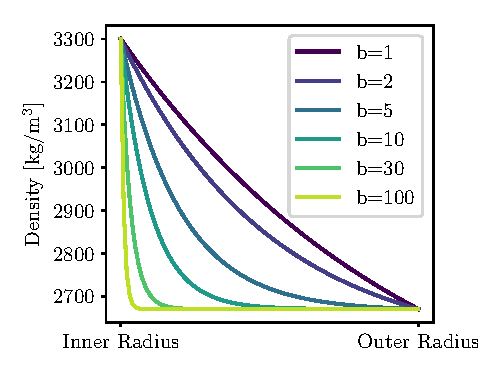
\includegraphics[width=\linewidth]{figs/tesseroids-variable-density/exponential-densities.pdf}
%}{
%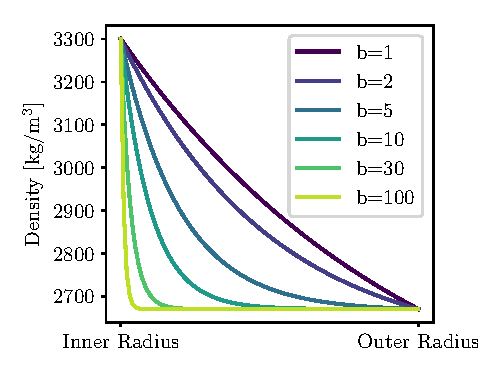
\includegraphics[width=0.5\linewidth]{figs/tesseroids-variable-density/exponential-densities.pdf}
%}
\caption{
    Exponential density functions assigned to the spherical shell models for
    $\delta$ ratio determination.
    Each density function corresponds to a different value of $b$ on
    Eq.~\ref{eq:density-exp}.
}
\label{fig:exp-densities}
\end{figure}


\subsubsection{$D$-$\delta$ space exploration}

We aim to find a combination of the $D$ and $\delta$ that produces a numerical error
lower than the 0.1\% threshold while minimizing computation time.
We use a grid search method and compute the numerical error for every ($D$, $\delta$)
pair belonging to a grid on the $D$-$\delta$ space (Fig.~\ref{fig:grid-search}).
For optimum algorithm performance, we search for the ($D$, $\delta$) pair that minimizes
the number of tesseroid division while keeping a numerical error under the 0.1\%
threshold.
This requirement translates into the smallest possible value of $D$ and the highest
possible value of $\delta$.

Because this is a time consuming computation, we limit the analysis to a high value of
$b=30$ (Fig.\ref{fig:exp-densities}) and the global grid defined in
Table~\ref{tab:grids}.
We compute the relative difference between the numerical and analytical results
of the gravitational potential ($V$) and its vertical derivative ($g_z$) for all shell
models defined in Table~\ref{tab:shell-models}.
For the sake of brevity, Fig.~\ref{fig:grid-search} shows the maximum difference values
obtained from all shell models.
The dotted lines in Fig.~\ref{fig:grid-search} represent a contour of 0.1\% relative
error.
Points inside the dotted are within the acceptable threshold.
Also shown in Fig.~\ref{fig:grid-search} are the $D$ values determined for the linear
density function in the previous section ($D_\text{linear}$).

The smallest values of $D$ that are within the 0.1\% threshold coincide with
$D_\text{linear}$ for both $V$ and $g_z$.
These results indicate that $D_\text{linear}$ can be safely extrapolated to non-linear
density cases.
This is not surprising considering that the two dimensional adaptive
discretization and the density-based discretization are independent of each other.
The former divides the tesseroid in the horizontal dimensions, while the latter only
divides in the radial dimension.
Hence, the optimal value of $\delta$ is likely to be independent of the optimal value of
$D$.
Because the grid search was limited to a specific computation grid and value of $b$,
we perform a more detailed analysis in the following section to determine an optimal
value of $\delta$ for the exponential density case.

\begin{figure}
\centering
%\iftwocol{
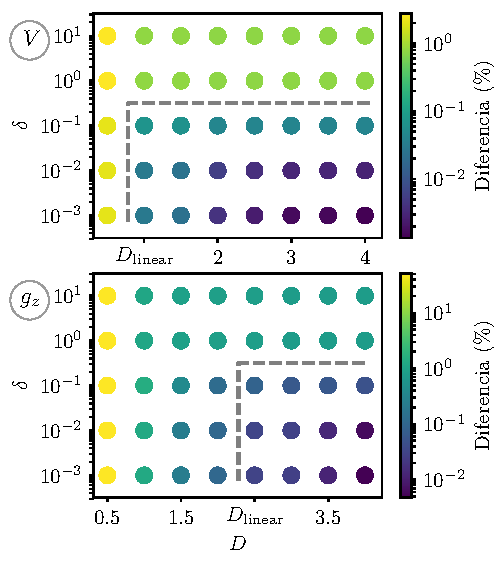
\includegraphics[width=\linewidth]
    {figs/tesseroids-variable-density/grid-search.pdf}
%}{
%\includegraphics[width=0.5\linewidth]
    %{figs/tesseroids-variable-density/grid-search.pdf}
%}
\caption{
    Numerical error exploration in the $D$-$\delta$ space.
    The percentage difference values were obtained from the comparison between the
    analytical solution and the numerical approximation of the gravitational fields ($V$
    and $g_z$) generated by a spherical shell with an exponential density function
    (Eq.~\ref{eq:density-exp}).
    These comparisons were carried out on the ``Global'' grid (Table~\ref{tab:grids}),
    with the spherical shell models detailed in Table~\ref{tab:shell-models}, and an
    exponential density function with $b = 30$.
    The percentage difference values are obtained as the maximum difference
    between every shell model.
    The points inside the dashed line are the ones that present an error lower than
    0.1\%.
    The $D$ value obtained for the linear density case for each gravitational field is
    also shown ($D_\text{linear}$).
    }
\label{fig:grid-search}
\end{figure}


\subsubsection{Delta ratio determination}

\begin{figure*}
\centering
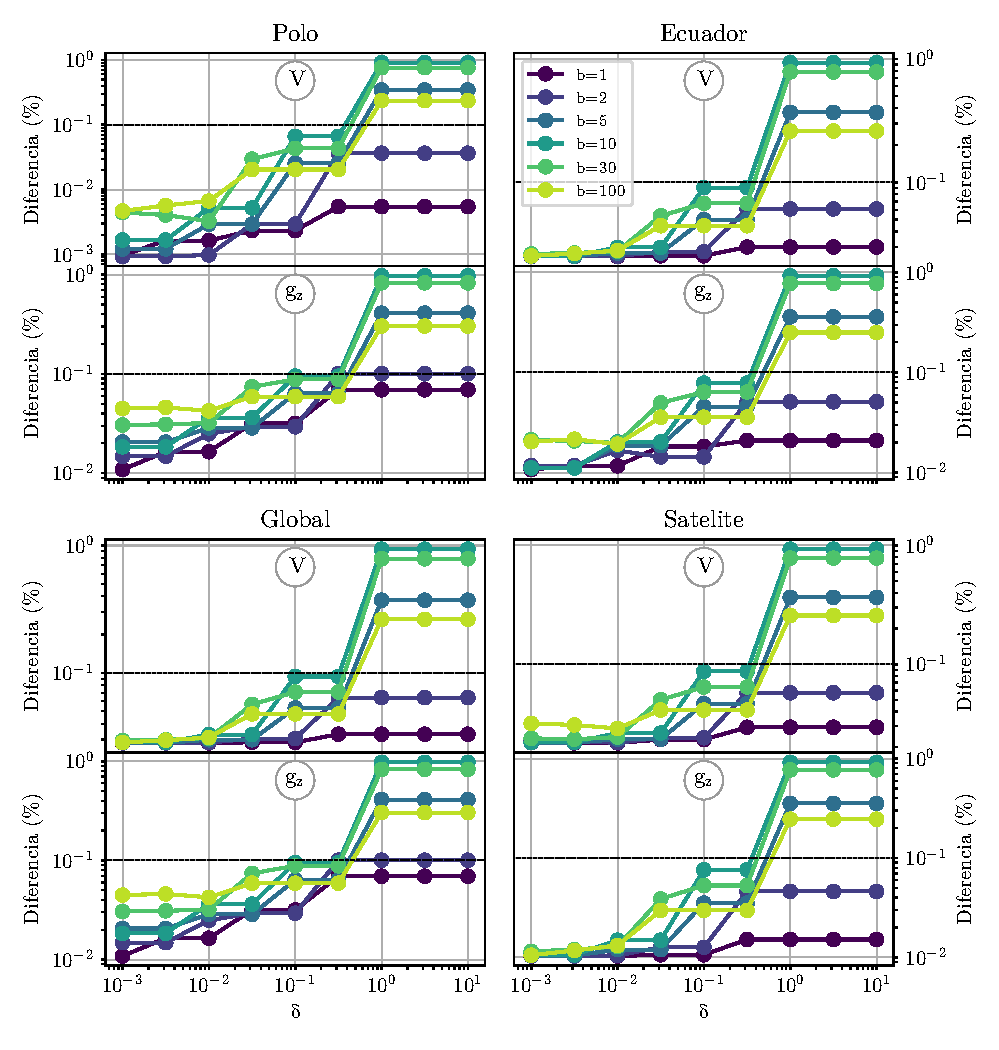
\includegraphics[width=\linewidth]{figs/tesseroids-variable-density/exponential-density-diffs.pdf}
\caption{
    Difference between the numerical and analytical solutions as a function of $\delta$
    ratio for different exponential density functions.
    These comparisons were carried out for every shell model
    (Table~\ref{tab:shell-models}) and computation grid (Table~\ref{tab:grids})
    using a fixed value of $D$.
    Each curve corresponds to the maximum difference out of all shell models
    for a particular value of $b$ (Eq.~\ref{eq:density-exp}).
    Differences are reported as a percentage of the analytical solutions.
    The horizontal dashed black line represents a target difference of 0.1\%.
    }
\label{fig:delta-exponential}
\end{figure*}

Having chosen values of $D$ equal to the ones obtained for the linear density case, we
are free to explore the integration error as a function of $\delta$ in more detail.
We will compute the difference between the numerical and analytical results for all
combinations of computation grid (Table~\ref{tab:grids}) and spherical shell model
(Table~\ref{tab:shell-models}), varying $\delta$ from $10^{-3}$ to $10^{1}$.
The calculations are repeated for each $b \in \{1, 2, 5, 10, 30, 100\}$
(Fig.~\ref{fig:exp-densities}) to examine the accuracy of the method for density
functions of different sharpness.
Because larger $\delta$ values result in fewer tesseroid divisions,
our intention is to find the highest value of $\delta$ that produces a relative
difference bellow the $0.1\%$ threshold.

Fig.~\ref{fig:delta-exponential} shows the resulting relative
differences for $V$ and $g_z$ as a function of $\delta$.
For the sake of brevity, each curve corresponds to the maximum difference between all
shell models.
The curves for $b=1$ and $b=2$ are below the 0.1\% threshold for all values of $\delta$
and do not change for $\delta > 0.8$, indicating that the density
functions are sufficiently smooth and no density discretizations are necessary.
For all other values of $b$, the difference falls below the 0.1\% threshold
if $\delta = 0.1$.
These results indicate that there is no significant relationship between the
sharpness of the exponential density function and the numerical error.


\subsection{Sinusoidal Density}

So far we have tested the density-based discretization algorithm against linear and
exponential density functions.
Nevertheless, this new algorithm is well suited to more complex continuous functions,
for example non-monotonic functions or those with multiple inflection points.
Although such density functions are rarely, if ever, seen in geological structures,
we want to subject our algorithm to such cases in order to show that it can solve more
complex situations than linear and exponential functions.
Furthermore, acquiring an optimal value for the $\delta$ ratio in case of unrealistic
density functions allow to extrapolate it to simpler realistic cases.
Thus this tests are only intended to submit the algorithm to the extreme and not to
emulate a real case scenario.

We will consider spherical shells with a sinusoidal density function defined as follows:

\begin{equation}
    \rho(r') = A \sin \left( 2 \pi b \frac{r' - R}{R_2 - R_1} \right) + A,
    \label{eq:density-sine}
\end{equation}

\noindent in which $A$ is a constant that controls the amplitude and vertical shift of
the sine function, $R$ is the mean Earth radius, and $b$ is a dimensionless constant
that regulates how many periods of the trigonometric function are included inside the
inner and outer radii.
The analytical solutions for $V$ and $g_z$ of a spherical shell with a sinusoidal
density function can be found on Appendix~\ref{cha:shell}.

We compute the relative difference between the numerical and analytical results for $V$
and $g_z$ for all combinations of spherical shell models (Table~\ref{tab:shell-models})
and computation grids (Table~\ref{tab:grids}).
We fixed the distance-size ratio $D$ to the ones obtained for the linear density case
and explored values of $\delta$ ranging from $10^{-4}$ to $1$.
The calculations are repeated for values of $b$ equal to 1, 2, 5 and 10
(Fig.~\ref{fig:sine-densities}).
For all computations, the value of $A$ is fixed at 1650 kg/m$^3$.

\begin{figure}
\centering
%\iftwocol{
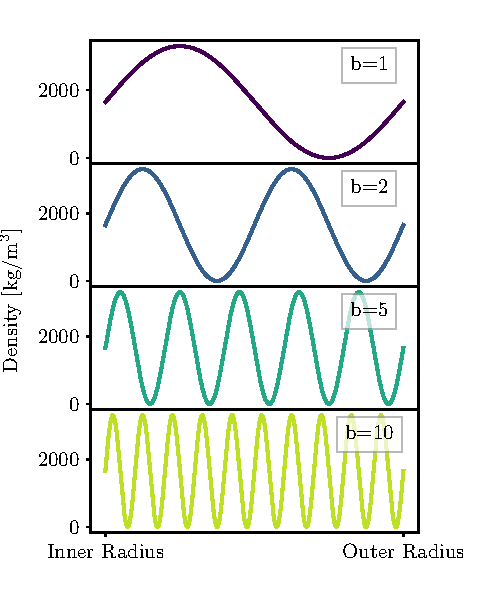
\includegraphics[width=\linewidth]{figs/tesseroids-variable-density/sine-densities.pdf}
%}{
%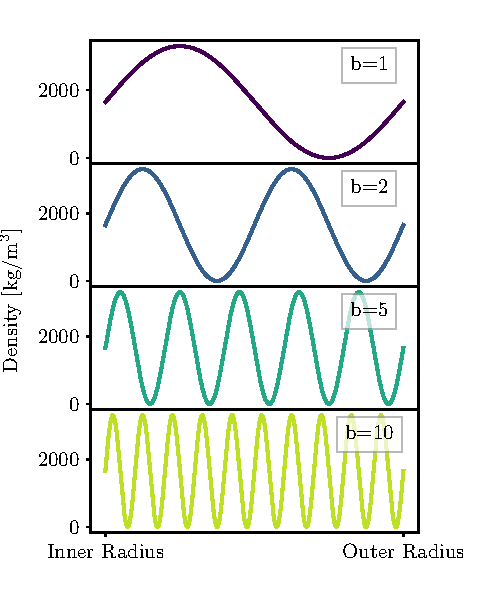
\includegraphics[width=0.5\linewidth]{figs/tesseroids-variable-density/sine-densities.pdf}
%}
\caption{
    Sinusoidal density functions assigned to the spherical shells in the $\delta$ ratio
    determination.
    Each density function corresponds to a different value of $b$ on
    Eq.~\ref{eq:density-sine}.
}
\label{fig:sine-densities}
\end{figure}

\begin{figure*}
\centering
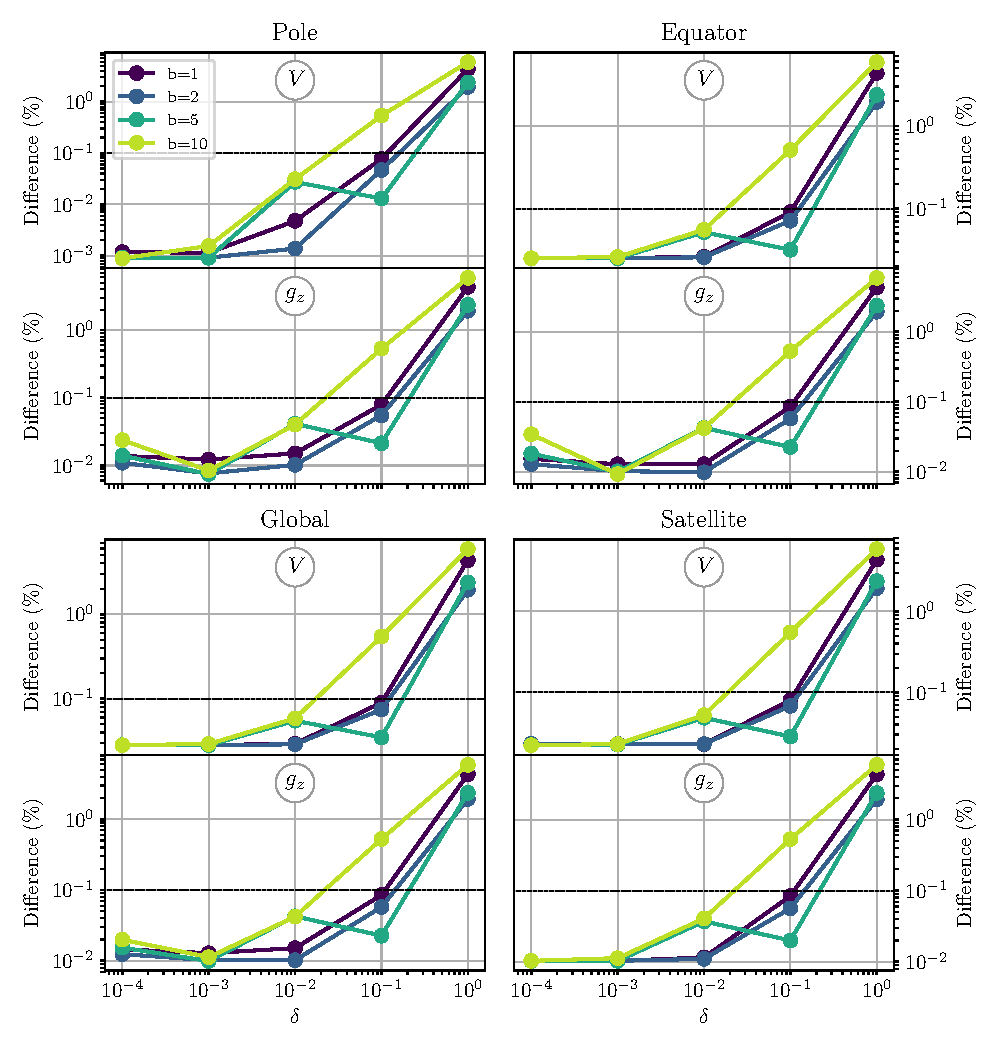
\includegraphics[width=\linewidth]{figs/tesseroids-variable-density/sine-density-diffs.pdf}
\caption{
    Difference between the numerical and analytical solutions as a function of $\delta$
    ratio for different sinusoidal density functions.
    These comparisons were carried out for every shell model
    (Table~\ref{tab:shell-models}) and computation grid (Table~\ref{tab:grids})
    using a fixed value of $D$.
    Each curve corresponds to the maximum difference out of all shell models
    for a particular value of $b$ (Eq.~\ref{eq:density-sine}).
    Differences are reported as a percentage of the analytical solutions.
    The horizontal dashed black line represents a target difference of 0.1\%.
    }
\label{fig:delta-sine}
\end{figure*}

Fig.~\ref{fig:delta-sine} shows the relative differences between the analytical
and the numerical solutions for sinusoidal density case.
Once again, each curve corresponds to the maximum difference between all shell models.
For all values of $b$ except for $b=10$,
the differences fall below the 0.1\% threshold for $\delta = 0.1$.
In the case of $b=10$, a lower value of $\delta = 0.01$ is required to achieve 0.1\%
difference.
We note that, even for the case of $b=10$, the differences for $\delta = 0.1$ are below
1\%.


%%%%%%%%%%%%%%%%%%%%%%%%%%%%%%%%%%%%%%%%%%%%%%%%%%%%%%%%%%%%%%%%%%%%%%%%%%%%%%%

\section{Algorithm performance}

Because the density-based discretization algorithm introduces more divisions along the
radial dimension, it is reasonable that the computation time for variable densities will
be higher than the homogeneous density case.
Directly comparing the computation time of both cases cannot be done in a meaningful
way because it is highly dependent on the implementation of the algorithm,
the choice of programming language, and the particular density function used.
In order to obtain an indicator of the increase in the computation time,
we chose the number of tesseroid divisions in the density-based discretization as a
proxy measure.

We analyse exponential density functions (Eq.~\ref{eq:density-exp}) with values of $b$
equal to 1, 2, 5, 10, 30 and 100, and sinusoidal density functions
(Eq.~\ref{eq:density-sine}) with values of $b$ equal to 1, 2, 5, and 10.
We then apply the density-based discretization algorithm on each function and record the
number divisions carried out.
Figs.~\ref{fig:number-of-tesseroids}a and~\ref{fig:number-of-tesseroids}b show the
exponential and sinusoidal density functions and the resulting discretization points as
orange dots.

For the exponential density functions, the algorithm performs a single division
independently of the value of $b$.
Therefore, the computation time would likely be at least twice that of the homogeneous
density case (assuming equal implementations).
On the other hand, Fig.~\ref{fig:number-of-tesseroids}c shows an almost linear relation
between the number of divisions in the sinusoidal density case and the value of $b$.
Thus, the computation time is likely to be dependent on the number of wavelengths
of the sinusoidal function that are contained within the tesseroid.

\begin{figure*}
\centering
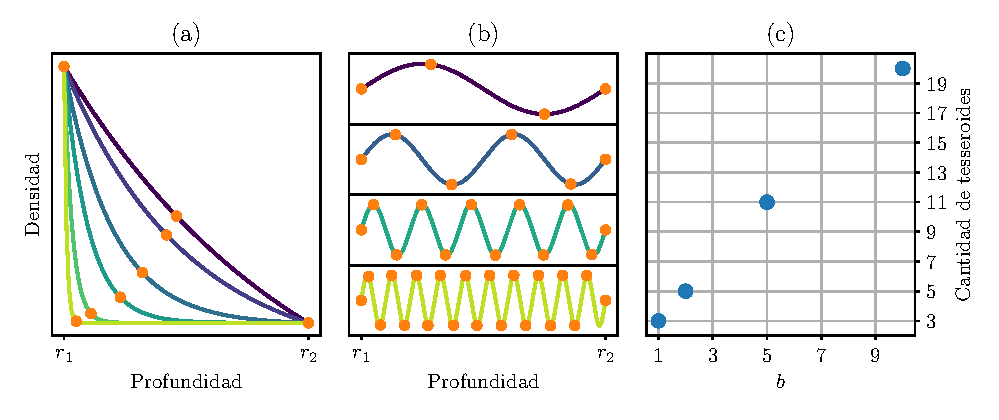
\includegraphics[width=\linewidth]{figs/tesseroids-variable-density/number-of-tesseroids.pdf}
\caption{
    Number of divisions performed by the density-based discretization algorithm
    (with $\delta = 0.1$) in case of
    (a)~exponential density functions with the same values of $b$ shown in
    Fig.~\ref{fig:exp-densities},
    (b)~sinusoidal density functions with the same values of $b$ shown in
    Fig.~\ref{fig:sine-densities}.
    On both figures, the locations of the tesseroid divisions are are marked with orange
    dots.
    (c) shows the number of discretized tesseroids for the sinusoidal density functions
    as a function of $b$.
}
\label{fig:number-of-tesseroids}
\end{figure*}


%%%%%%%%%%%%%%%%%%%%%%%%%%%%%%%%%%%%%%%%%%%%%%%%%%%%%%%%%%%%%%%%%%%%%%%%%%%%%%%

\section{Application to the Neuquén Basin}

We applied the new algorithms and optimal values of $D$ and $\delta$ determined
previously to calculate the gravitational effects of the Neuquén Basin,
a sedimentary basin located to the east of the Andes, between 32$^\circ$S and
40$^\circ$S latitude (Fig.~\ref{fig:neuquen-basin}a).
The basin includes continental and marine siliciclastics, carbonates, and evaporites
accumulated over the Jurassic and the Cretaceous constituting a stratigraphic record up
to 5000m of depth \citep{howell2005}.

\begin{figure*}
\centering
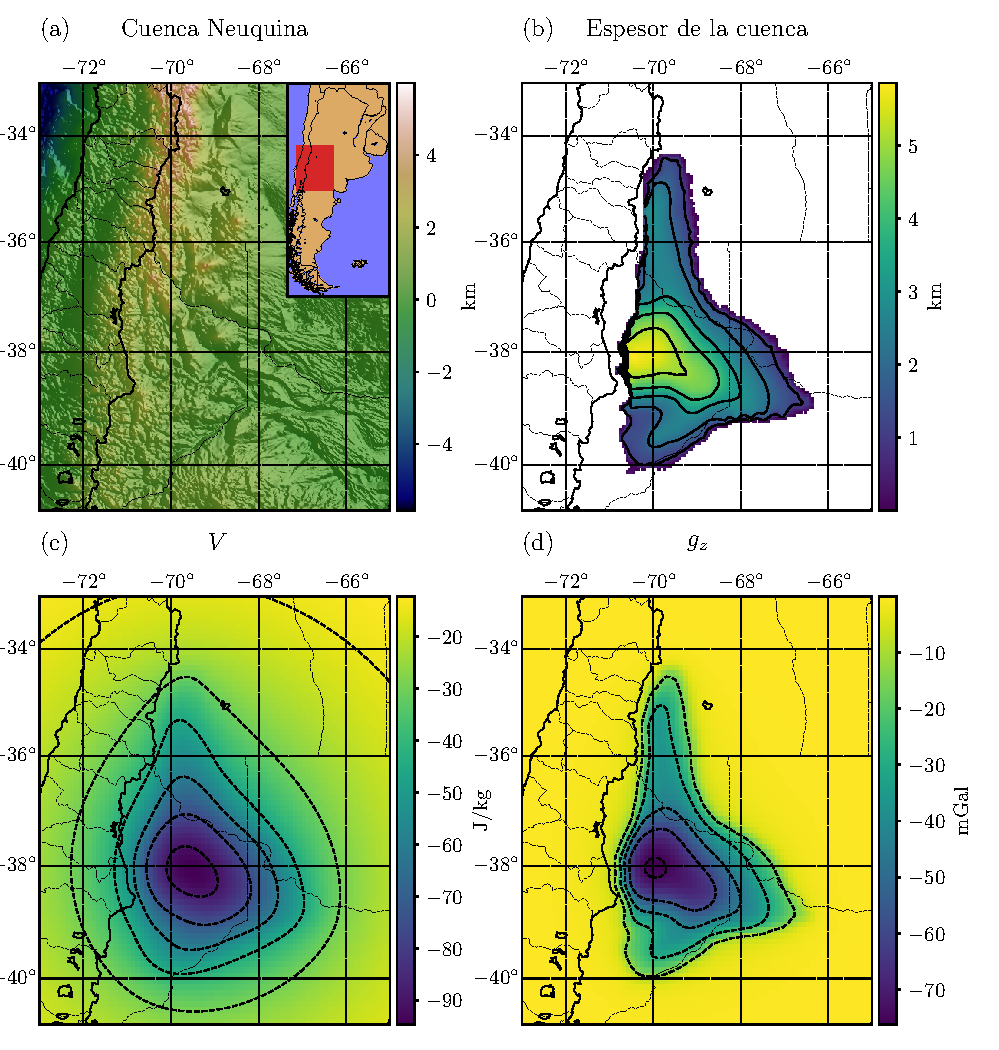
\includegraphics[width=\linewidth]{figs/tesseroids-variable-density/neuquen-basin.pdf}
\caption{
    Gravitational effects of the Neuquén sedimentary basin modelled
    using tesseroids with an exponential density function of depth.
    (a)~Topography of the Neuquén Basin (in km) and its location in South America,
    (b)~thickness of the sedimentary basin \citep[in meters;][]{heine2007},
    (c)~resulting gravitational potential $V$,
    (d)~resulting vertical component of the gradient ($g_z$),
    calculated at 10km of height over the mean Earth radius.
}
\label{fig:neuquen-basin}
\end{figure*}

\begin{figure}
\centering
%\iftwocol{
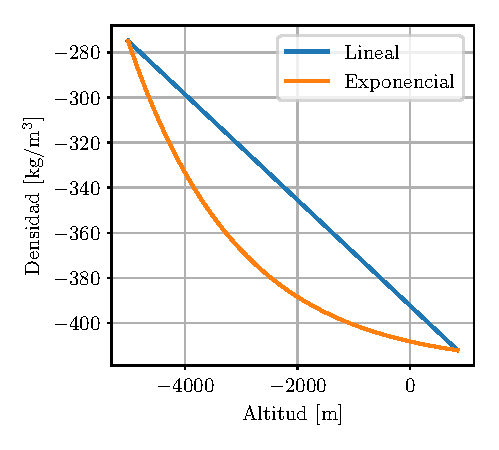
\includegraphics[width=\linewidth]{figs/tesseroids-variable-density/neuquen-basin-densities.pdf}
%}{
%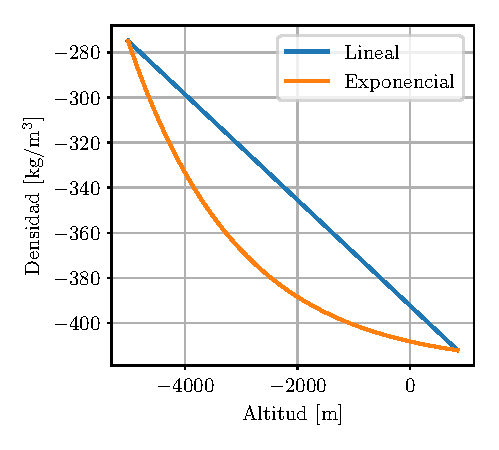
\includegraphics[width=0.5\linewidth]{figs/tesseroids-variable-density/neuquen-basin-densities.pdf}
%}
\caption{
    Linear and exponential densities used to compute the gravitational fields generated
    by a tesseroid model of the Neuquén sedimentary basin.
    The height is defined above the mean Earth radius, and its axis is spanned between
    the deepest and the highest point of the basin.
}
\label{fig:neuquen-basin-densities}
\end{figure}


\begin{figure*}
\centering
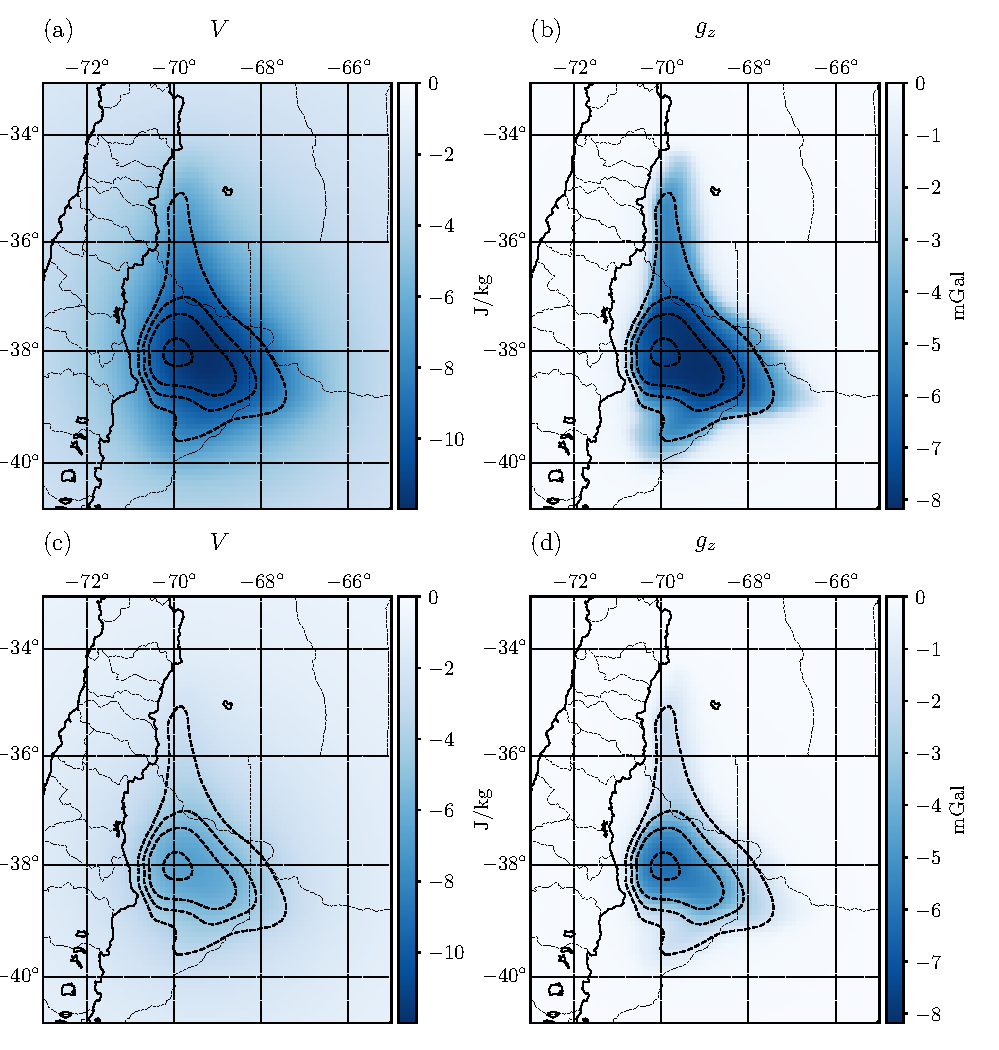
\includegraphics[width=\linewidth]{figs/tesseroids-variable-density/neuquen-basin-diffs.pdf}
\caption{
    Differences between the gravitational fields generated by the tesseroid model of the
    Neuquén basin with an exponential density contrast and with a homogeneous and
    linear density variation.
    \mbox{(a)-(b)}~Differences on $V$ and $g_z$ between the exponential density model
    and the homogeneous density one,
    \mbox{(c)-(f)}~differences on $V$ and $g_z$ between the exponential density model
    and the linear density one, calculated at 10km of height over the mean Earth radius.
}
\label{fig:neuquen-basin-diffs}
\end{figure*}

The thickness of the sediment pack was digitized from \citet{heine2007} on a regular
grid with a resolution of 0.05$^\circ$ on both longitude and latitude directions
(Fig.~\ref{fig:neuquen-basin}b).
We created a tesseroid model of the sediment pack by placing a
$0.05^\circ \times 0.05^\circ$ tesseroid on each node of the grid.
The top of each tesseroid was fixed at the median of the topography of the basin
(845~m above mean Earth radius) and the bottom at corresponding thickness of the basin.

We must also define a density function for the tesseroid model.
\citet{sigismondi2012} measured a minimum and maximum density contrast for
the Neuquén basin of -412kg/m$^3$ and -275kg/m$^3$, respectively.
We have chosen an exponential density variation (Eq.~\ref{eq:density-exp}) that assumes
the minimum value on the top surface and the maximum at 5014m depth (the thickest part
of the basin), with a value of $b$ equal to 3.
This density variation is in the order of magnitude of the ones used by
\citet{cowie1990} and \citet{cordell1973}.
This density function can be seen on Fig.~\ref{fig:neuquen-basin-densities}.

Finally, we computed the gravitational potential $V$ and the vertical component of the
gradient ($g_z$) on a computation grid of $159\times163$ nodes ($0.05^\circ$ spacing on
both longitude and latitude) at a 10 km height over the mean Earth radius.
The resulting fields can be seen in Fig.~\ref{fig:neuquen-basin}c-d.

We computed the differences between the results for the exponential density function and
those generated by the same model but now with a constant density (the mean of
-412kg/m$^3$ and -275kg/m$^3$).
We also computed the differences between the exponential density and a linear density
that assumes these two values on the highest and the deepest point of the basin
(Fig.~\ref{fig:neuquen-basin-densities}).
Fig.~\ref{fig:neuquen-basin-diffs}a-b and Fig.~\ref{fig:neuquen-basin-diffs}c-d show the
differences with the constant and the linear density, respectively.
The maximum absolute difference in the computed $g_z$ is approximately 8 mGal for the
homogeneous case and approximately 6 mGal for the linear density case.
Both are well above the accuracy of most available data products.


%%%%%%%%%%%%%%%%%%%%%%%%%%%%%%%%%%%%%%%%%%%%%%%%%%%%%%%%%%%%%%%%%%%%%%%%%%%%%%%

\section{Discussion}

By including the density function into the GLQ integration, the method described here
can be applied without modification to tesseroids with density following any continuous
function of radius.
A density-based discretization algorithm divides the tesseroid in the radial dimension
to ensure accurate integration of the density function.
This algorithm is independent of the GLQ integration and could potentially be used to
determine an optimal discretization when approximating a density function by piecewise
linear \citep{lin2019} or piecewise polynomial \citep{fukushima2018} functions.

Our numerical experiments show that the two dimensional adaptive discretization is
enough to achieve 0.1\% accuracy with a second-order GLQ in the case of a linear density
function (Fig.~\ref{fig:D-linear}).
Values of the distance-size ratio determined here for the gravitational potential
($D=1$) and its vertical derivative ($D=2.5$) are compatible with \citet{uieda2016}.
These results also show that there is no significant relationship between the accuracy
of the method and the thickness of the tesseroid model.

The $D$-$\delta$ space exploration for the exponential density function
(Fig.~\ref{fig:grid-search}) showed that values of $D$ determined for the linear density
case are equally applicable to the exponential density case.
Furthermore, the difference with respect to the analytical solution only falls below
0.1\% for values of $\delta$ lower than 0.1.
It follows that the density-based discretization is required to achieve the desired
accuracy level for non-linear density functions.

More detailed error analyses showed that $\delta = 0.1$ is sufficient to guarantee an
accuracy of 0.1\% for all exponential density functions tested
(Fig.~\ref{fig:delta-exponential})
and most of the sinusoidal functions tested (Fig.~\ref{fig:delta-sine}).
The exception is the case of a sinusoidal function with $b = 10$
(Eq.~\ref{eq:density-sine}), for which $\delta = 0.01$ is required to achieve 0.1\%
accuracy.
Nevertheless, using $\delta = 0.1$ in this case would still produce results with an
error of less than 1\%.

While the algorithms proposed here can be applied to any continuous density function,
the optimal values for $D$ and $\delta$ are empirically determined only for linear,
exponential, and sinusoidal density functions.
Thus, we can only say with certainty that these values will produce results with 0.1\%
accuracy for these functions.
However, all of our numerical tests include worse-case scenarios (zero computation
heights, large tesseroids, highly variable density functions, etc).
For this reason, these optimal values of $D$ and $\delta$ can plausibly be
extrapolated to any realistic continuous density function.
Notwithstanding, we encourage users of the algorithms and software to perform similar
tests in order evaluate the accuracy when using density functions more complex than the
ones tested here.

The algorithm performance analysis shows that the computation time using variable
densities is likely to be at least two times larger than the homogeneous density case.
It is also likely to increase proportionally to the number of inflection points of the
density function.
As is the case for most numerical methods, there is a trade-off between computation time
and accuracy.
Nevertheless, density profiles will have few inflection points for most geophysical
applications.
Therefore, the computation time would be in the same order of
magnitude as the one for the homogeneous density in most real world applications.

%%%%%%%%%%%%%%%%%%%%%%%%%%%%%%%%%%%%%%%%%%%%%%%%%%%%%%%%%%%%%%%%%%%%%%%%%%%%%%%

\section{Conclusions}

We have developed a new methodology to compute the gravitational potential and its
gradient for a tesseroid with a density given by a continuous function of radius.
It numerically solves the volume integrals through Gauss-Legendre Quadrature (GLQ) by
including the density function in the numerical integration.
By implementing the algorithm in the dynamic Python programming language, users can
define their own density function to supply to the software.
This allows the use of any arbitrary continuous function without modification to the
method or software.
The accuracy of the numerical integration is automatically controlled by a two
dimensional adaptive discretization algorithm and a new density-based discretization
algorithm.
The former divides the tesseroid in half if the ratios of the distance to the
computation point and the latitudinal or the longitudinal size of the tesseroid are
smaller than a predefined distance-size ratio $D$.
This algorithm minimises the integration error when the computation point is close to
the tesseroid.
Nevertheless, the adaptive discretization alone is not sufficient to guarantee the
accuracy of the method in case of tesseroids with non-linear density functions.
To overcome this challenge, the density-based discretization algorithm
divides the tesseroid along the radial dimension on the points at which the maximum
variations of the density function take place.
The number of radial divisions performed, and thus the accuracy of the computation, is
controlled by the $\delta$ parameter.
This new algorithm is intended to minimise the error due to the inability of
the GLQ to produce precise approximations of density functions with sharp variations.

We empirically determined optimal values for $D$ and $\delta$ by comparing the numerical
results with analytical solutions.
Our analysis included a range of tesseroid models and computation grids as well as
common density functions.
These values minimize the computational load while maintaining the numerical error below
0.1\% of an analytical solution.
The density functions used to establish the optimal values were a linear, an
exponential, and a sinusoidal function.
The linear function represents the smoothest variation of density and does not require
density-based discretization at all.
Through this analysis, we have obtained optimal values for the distance-size ratio $D$
of 1 and 2.5 for the potential and its gradient, respectively.
We analysed the error for exponential functions ranging from smooth to sharp and
sinusoidal function of different wavelengths to test the accuracy of the density-based
discretization.
It worth noting that the sinusoidal density tests were carried out in order to test the
algorithm to the extreme and not to emulate a real world scenario.
Values of $\delta$ equal to 0.1 are sufficient to guarantee a 0.1\% accuracy for most
realist cases tested.
These results could be extrapolated to other continuous density functions that are
sufficiently smooth, as is the case for most common geophysical applications.
Smaller values of $\delta$ can be used for more highly variable density functions to
increase the accuracy of the integration accordingly.

Some computational performance is sacrificed in order to obtain an accurate and general
purpose method.
The density-based discretization adds to the computation time by increasing
the number of GLQ integrations.
Likewise, allowing users to supply custom density functions incurs an overhead cost
because of the added function evaluations.
It is also impossible to optimize the source code and formulas without knowledge of the
specific density function.
Nonetheless, the density-based discretization is independent of the adaptive
discretization and GLQ integration.
It can be viewed as a type of pre-processing step that can be combined with other more
specialized integration methods.

An application to modelling the Neuquén Basin, Argentina, demonstrates that the
effects of sediment compaction cannot be ignored.
When compared to an exponential density function, a homogeneous density with depth would
result in an error of up to -8 mGal, while a linear density function would result in up
to -6 mGal error.
Accurate and robust forward modelling is a key component to any gravity inversion
method.
Errors of this magnitude could result in significant overestimation of sedimentary
basin thickness, for example.



%%%%%%%%%%%%%%%%%%%%%%%%%%%%%%%%%%%%%%%%%%%%%%%%%%%%%%%%%%%%%%%%%%%%%%%%%%%%%%%

\section{Acknowledgments}

We are indebted to the developers and maintainers of the open-source software without
which this work would not have been possible.
We would also like to thank editor Kosuke Heki and two anonymous reviewers for their
comments and contributions.
This is SOEST contribution 10717.
